\documentclass[tikz]{standalone}
\usepackage{tikz}
\usetikzlibrary{calc,arrows.meta}

\begin{document}
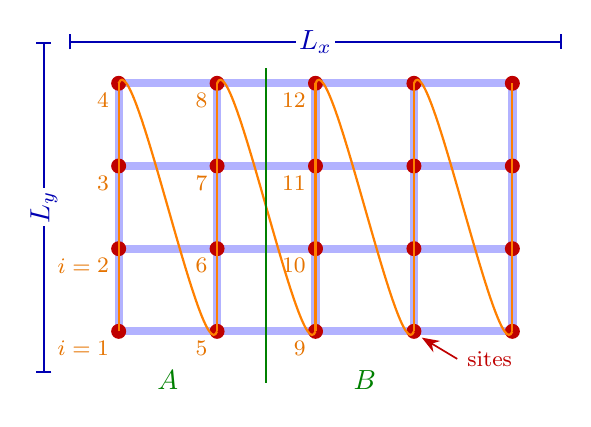
\begin{tikzpicture}[
	site/.style={
		circle,
		fill=red!75!black,
		draw=red!75!black,
		inner sep=0pt,
		minimum size=5pt
	},
	gridline/.style={blue!30!white,line width=3pt},
	pathline/.style={orange, thick},
	partline/.style={green!50!black, semithick},
	dimline/.style={blue!70!black, semithick},
]

\pgfmathsetmacro{\ncols}{5}
\pgfmathsetmacro{\nrows}{4}
\pgfmathsetmacro{\dx}{1.25}
\pgfmathsetmacro{\dy}{1.05}
\pgfmathsetmacro{\ncolsm}{\ncols-1}
\pgfmathsetmacro{\nrowsm}{\nrows-1}
\pgfmathsetmacro{\gridW}{\ncolsm*\dx}
\pgfmathsetmacro{\gridH}{\nrowsm*\dy}
\pgfmathsetmacro{\partX}{1.5*\dx}

% grid
\foreach \x in {0,...,\ncolsm} {
	\draw[gridline] (\x*\dx, 0) -- (\x*\dx, \gridH);
}
\foreach \y in {0,...,\nrowsm} {
	\draw[gridline] (0, \y*\dy) -- (\gridW, \y*\dy);
}

% sites and numbering (first three columns as on the board)
\foreach \x in {0,...,\ncolsm} {
	\foreach \y in {0,...,\nrowsm} {
		\pgfmathtruncatemacro{\snum}{\x*4+\y+1}
		\coordinate (s\x\y) at (\x*\dx, \y*\dy);
		\node[site] at (s\x\y) {};
		\ifnum\x<3
			\node[orange!90!black, font=\footnotesize, below left] at (s\x\y) {\snum};
		\fi
	}
}

% snake path: up each column, curved jump to next column
\foreach \x in {0,...,\ncolsm} {
	\draw[pathline] (s\x0) -- (s\x\nrowsm);
}
\foreach \x in {0,...,\nrowsm} {
	\pgfmathtruncatemacro{\xp}{\x+1}
	\draw[pathline]
		(\x*\dx, \gridH) % to [out=90,in=270]
		.. controls (\x*\dx + 0.2, \gridH + 0.5*\dy) and (\xp*\dx-0.2, -0.5*\dy) ..
		% .. controls (\x*\dx+0.55*\dx, \gridH+0.55) and (\xp*\dx-0.30*\dx, -0.55) ..
		 (\xp*\dx, 0);
}

% row indices on the left of the first column
\node[orange!90!black, font=\footnotesize, below left] at (s00) {$i=\phantom{1}$};
\node[orange!90!black, font=\footnotesize, below left] at (s01) {$i=\phantom{2}$};

% bipartition A | B
\draw[partline] (\partX, -0.65) -- (\partX, \gridH+0.20);
\node[green!50!black] at ({\partX - \dx}, -0.62) {$A$};
\node[green!50!black] at ({\partX + \dx}, -0.62) {$B$};

% dimensions
\draw[dimline, |-|] ({-0.5*\dx},{\gridH+0.5*\dy}) -- ({\gridW+ 0.5*\dx}, {\gridH+0.5*\dy})
	node[midway, fill=white, inner sep=1pt] {$L_x$};
\draw[dimline, |-|] (-0.95, {-0.5*\dy}) -- (-0.95, {\gridH + 0.5*\dy})
	node[midway, fill=white, inner sep=1pt, sloped] {$L_y$};

% "sites" annotation
\draw[{Stealth[length=2.2mm]}-, red!75!black, semithick]
	 ($(s30)+(0.1,-0.08)$) --
	($(s30)+(0.55,-0.35)$) 
node[font=\footnotesize, right] {sites};

\end{tikzpicture}
\end{document}
